\documentclass{homework}
\usepackage{graphicx}

\title{ELEC400m Assignment 1}
\author{Matthew\ Sam}
\date{29/09/2022}

\begin{document}

\maketitle

\exercise
a)

In this question we find the optimal theta for the given linear model.
\[
\emph{f} _{\Theta}(x _{1}, x _{2}) = \theta _{0} + \theta _{1}x_{1}
\]
By leveraging the optimal solution for theta:
\[
(\bold{X}^{T}\bold{X})^{-1}\bold{X}^{T}Y
\]
Using this optimal theta, a line can be plotted using arbitrary data points (in my case I use 1-10)
\centering
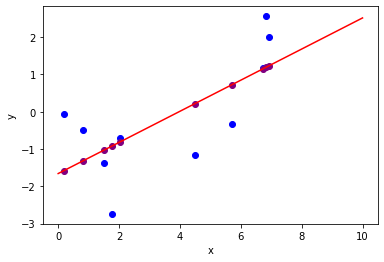
\includegraphics[width=250]{1a.png}

\caption{figure 1: line created from optimal theta}

\raggedright
b)

In this question, an additional input feature is added by squaring all values of x1
\centering
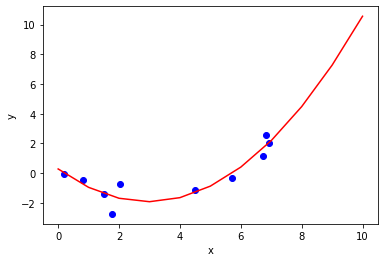
\includegraphics[width=250]{1b.png}

\caption{figure 2: using a similar method as 1a) but increasing the amount of features by 1}

\raggedright
c)

Similarly to question b), 2 more features are added: \(x^3\) and \(x^4\)

\centering
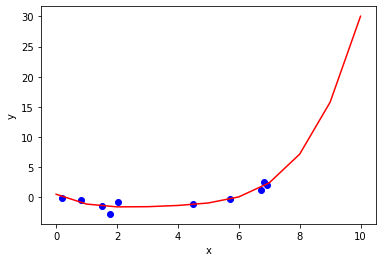
\includegraphics[width=250]{1c.png}

\caption{figure 2: using a similar method as 1a) but increasing the amount of features by 4}

\raggedright
d)

from looking at the data points I would say that having a line would result in under fitting as they do not appear to have a linear relationship. It's a bit harder to say for the next two functions used. function b and function c visually appear to have predicted y well in comparison to a which is to be expected. When viewed against the test data instead of the training data they both appear to perform similarly. My error assessment appears to support that both b and c perform similarly, with c having the slight edge on the test data. This leads me to believing that none of the functions are over fit.

e)

the SKLearn LinearRegression function was trained on the same training values that the analytic solution used for finding the optimal theta the resulting theta's were identical to those found using the analytic solution:

thetas from my model:
\[


for\ 1a:\
\begin{bmatrix}
 -1.65766519  0.41725154 
\end{bmatrix}


for\ 1b:\
\begin{bmatrix}
 0.28514264 -1.48968069  0.25172685 
\end{bmatrix}


for\ 1c:\
\begin{bmatrix}
 0.51817538 -2.52130644  1.07886107 -0.19978244  0.01466235
\end{bmatrix}
\]

thetas from SKL:
\[


for\ 1a:\
\begin{bmatrix}
 -1.65766519  0.41725154 
\end{bmatrix}


for\ 1b:\
\begin{bmatrix}
 0.28514264 -1.48968069  0.25172685 
\end{bmatrix}


for\ 1c:\
\begin{bmatrix}
 0.51817538 -2.52130644  1.07886107 -0.19978244  0.01466235
\end{bmatrix}
\]
\exercise*
a)

In the question we are given two equations:
\[
\emph{f} _{\Theta}(x _{1}, x _{2}) = \theta _{0} + \theta _{1}x_{1} + \theta _{2}x_{2}\ - linear\ model\
\]
\[
\sigma _{\Theta}(x _{1}, x _{2})  = \frac{1}{1+e^{\emph{f} _{\Theta}(x1, x2)}} - logistic\ regression\ classifier\ function\
\]
Binary cross entropy loss is defined by:
\[
    -y*ln(P(y))-(1-y)*ln(1-P(y))\ y\in(0,1)
\]

substituting out linear model into our logistic regression classifier yields our logistic model:
\[
P(\hat{y}|x _{1},x _{2}) = \frac{1}{1+e^{\theta _{0} + \theta _{1}x_{1} + \theta _{2}x_{2}}} 
\]

Substituting P into the cross-entropy loss formula gives us our cross-entropy error function
\[
    loss = -y*ln(\frac{1}{1+e^{\theta _{0} + \theta _{1}x_{1} + \theta _{2}x_{2}}})-(1-y)*ln(1-\frac{1}{1+e^{\theta _{0} + \theta _{1}x_{1} + \theta _{2}x_{2}}})
\]

b)

In order to update the theta starting values to their next iteration we can do the first step of the gradient descent summation on our starting theta values and given alpha:
\[
\theta _{0} = -1\
\theta _{1} = -1.5\
\theta _{2} = 1.5\
\alpha =0.1\
\]
\[
\Theta_{new}\leftarrow \Theta-\alpha\sum_{i=1}^{m} (1+e^{-\bold{X}^{(i)\bold{T}}\Theta}-y^{(i)})\bold{X}^{(i)}
\]
after doing one step through the for loop that calculates this summation, we get out new thetas as:
\[
\begin{bmatrix}
 -0.65014251\ -0.54681755\ 0.63228741\
\end{bmatrix}
\]

c)

The following figures illustrate the gradient descent model's hyperplane decision boundaries at initial conditions, one iteration, and after convergence

\centering
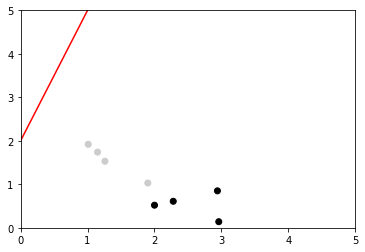
\includegraphics[width=250]{2b0.png}

\caption{figure 4: hyperplane with initial values}

\centering
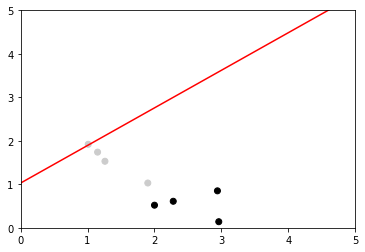
\includegraphics[width=250]{2b1.png}

\caption{figure 5: hyperplane after 1 iteration}

\centering
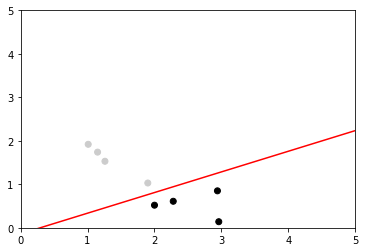
\includegraphics[width=250]{2bf.png}

\caption{figure 6: hyperplane after convergence}

\raggedright

d)

SKLearn's logistic regression implementation is trained on the same data-set as the gradient descent model, and given the parameters of 50000 max iterations, and no penalty. It produced a set of thetas:
\[
\begin{bmatrix}
 -2.91576747\ 15.90678769\ -35.93982465\
\end{bmatrix}
\]

e)

The output of the SKLear model and gradient descent model were evaluated by measuring their accuracy, precision, and sensitivity. The following formulas were used to calculate these values:

\[
Precision = \frac{TP+TN}{TP+FP+FN+TN}
\]

\[
Accuracy = \frac{TP}{TP+FP}
\]

\[
Sensitivity = \frac{TP}{FP+FN}
\]
The resulting calculated metrics showed that the two models had identical performance across the test data=-set.
metrics GD: 

\    accuracy:  0.8333333333333334
    
\    precision:  1.0
    
\    sensitivity:  0.4
    
metrics SKL: 

\    accuracy:  0.8333333333333334
    
\    precision:  1.0
    
\    sensitivity:  0.4
\end{document}
